\part*{Lecture 6: Forward Volatility, Caps, Floors, and Swaptions}
\addcontentsline{toc}{part}{Lecture 6: Forward Volatility, Caps, Floors, and Swaptions}
\beginlecture{06}

Lecture~6 opens with the lecturer announcing the plan for the day:
``today we're going to discuss briefly the Freddie Mac callable bond
case, give a few wrap-up thoughts there \ldots\ then we will be jumping
in today to, our biggest topic is forward volatility.\ That's going to
get us deep into the three big products of forward volatility, caps,
floors, and swaptions.'' The first hour of the session is therefore a
deliberate revisit of the Lecture~5 case study (model price, OAS,
duration of a callable, and the implied-vol-of-rate vs.\
implied-vol-of-price translation), with the lecturer using student
questions to surface every approximation that went into the
\$98.67 model number against the \$100.09 market quote. Only after
that does the class pivot --- via a short Q\&A on Bloomberg's
normal-vol toggle and a coffee break --- into the new chapter
\emph{7.1~Forward Volatility and Caps} and the companion notebook
\emph{7.2~Swaptions}. The notes below preserve that order.

Two structural points are worth flagging up front. First, ``forward
volatility'' is the punchline of this lecture, and the analogy to
beat into the ground is \emph{flat~vol is to forward~vol as YTM is to
the spot curve} --- a student volunteers exactly that line on the
first try and the lecturer cheerfully concedes ``you just grabbed the
punchline.'' Second, the exact same Black-formula machinery from
Lecture~5 carries over to caps, floors, and swaptions; what changes
between products is only \emph{which} forward rate (a single quarterly
forward, a single annual swap rate, or a forward swap rate) goes in
where the underlying used to be. Under that lens caps, floors, and
swaptions are the call/put toolkit for the world of swaps and forward
swaps, the same way ordinary equity calls and puts are the toolkit
for stocks.

\section{Closing the Freddie Mac case study}\label{L6-sec:freddie}

The lecturer opened by noting why he wanted to belabor the case one
more session: ``I'll be surprised if any of you go into market making
agency bonds like Freddie Mac.\ If you do, please come back as guest
speaker.'' The point is not the product. The point is that the
callable bond is a clean bridge from the Black--Scholes setup of
FINMAT~330 (a single asset, a single rate, lognormal returns) into
fixed-income derivatives (a curve of rates, an underlying that
changes shape over the option's life, and a Black-formula recipe in
which the discount factor and the variance accrual reference different
points in time). He also reminded the room that the issues he had
the class price are very small --- ``less than 100~million for all
three combined'' --- so the case is pedagogical, not commercial.

\subsection{Setup of the simplified bond}\label{L6-sec:freddie-setup}

\begin{keyblock}
\textbf{Cells (Page \emph{Case Study --- Freddie Mac Bonds}).}
\emph{(Bond info, simplified.)}\\
The example bond is a Freddie~Mac callable issued in early 2025, with
\begin{itemize}
  \item maturity 2030 (about 5~years from quote date),
  \item first call date in 2028 (about 3~years from now),
  \item coupon $4.41\%$ paid semiannually, notional 10~million.
\end{itemize}
For the case the option is treated as \textbf{European} with a single
exercise at $T_o = 3$~years, even though the actual contract is
\textbf{Bermudan}. The underlying that would be delivered if the
option is exercised is therefore not the original 5-year bond but a
\textbf{2-year bond} starting at $T_o$.
\end{keyblock}

The lecturer pressed two questions in sequence on this slide: ``what
kind of maturity are we talking about on this bond?'' (5~years) and
``when is it callable?'' (3~years). With the European simplification,
the only date that matters for Black's formula is the option
expiration $T_o = 3$, and at that date the bond left to deliver has
$T_{\text{bond}} - T_o = 2$ years remaining. ``You always are having
to keep track of the fact that this is a five-year bond right now,
but given that it's an expiration of three years, at that point, it
will be a two-year bond.'' The lecturer was explicit that the
European simplification will tend to push the model price of the
callable \emph{up} relative to the truth: a Bermudan exercise gives
the issuer more flexibility, which makes the embedded short call
worth more, and a more valuable embedded short call drives the
callable price down. ``It wouldn't be 98.67. It'd be even lower.''
The class will revisit the Bermudan correction in a later lecture
when numerical methods are on the table.

The discount curve handed to the class for the case was \emph{built
from swaps}, not Treasuries. The lecturer made the class debate the
choice openly: swaps win on liquidity, especially at long maturities,
but the Freddie~Mac cash flows have agency credit risk while the
cleared swap curve has almost none, and in 2008-onward the agencies
have been run by the Treasury, so a Treasury curve might be the more
honest benchmark. ``Maybe we should use a Treasury curve. On the
other hand, the Treasury curves have their own problems with
specialness for liquidity, which this definitely doesn't have.''
The case takes the swap curve and notes the mismatch openly, rather
than pretending the choice is clean.

\begin{checkpoint}
\textbf{My note.} The recurring theme from Week~1 (\emph{step one is
always: get a curve you trust}) returns here in a more uncomfortable
form. There is no curve that is exactly right for this bond. The
callable Freddie~Mac is not a swap, not a Treasury, and not a
corporate; it sits in the gap between the swap curve and the
Treasury curve, and the OAS we will compute below is partly a
statement about the bond and partly a statement about which curve
we used. The lecturer's framing --- ``part of it is explained by our
rate construction, part of it is explained by suboptimal exercise''
--- is the pragmatic answer.
\end{checkpoint}

\subsection{Why Black, not Black--Scholes}\label{L6-sec:freddie-blackvsbs}

\begin{keyblock}
\textbf{Quick recap.} Black--Scholes is a poor model here for two
reasons:
\begin{itemize}
  \item It assumes a \emph{flat term structure that never changes}.
        ``If we have a flat term structure that never changes, then
        what do we need to do? End class, right?''
  \item It assumes \emph{Brownian price dynamics for the underlying
        bond}, but a bond's clean price is mechanically pulled to
        par at maturity, and the dirty price has predictable jumps
        on coupon dates.
\end{itemize}
Black's formula does not solve the second problem cleanly --- bond
prices still misbehave under lognormal dynamics --- but it patches it
substantially by replacing the \emph{spot} price with the \emph{forward}
price, which absorbs the predictable carry-and-coupon part of the
drift.
\end{keyblock}

The lecturer's framing here was that Black's formula is not an
endorsement of lognormal bond prices; it is the cheapest possible
patch on Black--Scholes that lets the FINMAT~330 toolkit survive
contact with a bond. ``We're not really going to solve this issue.
The bond prices have some predictability. If we use Black's formula,
we're still assuming that Brownian motion. So I should be clear that
that's not going to save us from that. But what will help is that
we're going to use clean prices.'' Combined with the move from spot
price to forward price, the predictable drops on coupon dates are
absorbed into the carry term and the residual is closer to (though
not exactly) a Brownian-like process.

\subsection{The forward price in this problem: a 3-year forward on a
2-year bond}\label{L6-sec:freddie-fwd}

\begin{keyblock}
\textbf{What forward do we need?}
A forward always references two dates: the date the contract is
signed and the date it is delivered. For Black's formula on this
callable, the underlying at exercise is a \textbf{2-year bond} (since
$T_{\text{bond}} - T_o = 5 - 3 = 2$), and the contract is signed
\emph{today}. The number we need is therefore the
\textbf{3-year forward price of the 2-year bond}, computed from the
no-arbitrage forward formula of Lecture~4:
\[
  P_{\text{fwd}}(0,T_o,T_{\text{bond}})
    \;=\; \frac{P(0)\;-\;\sum_{T_i \in (0, T_o]} c_i\, Z(0,T_i)}{Z(0,T_o)}.
\]
With the discount curve handed to the class and the contractual coupon
schedule, the formula returns about $\$100.50$ for the
3-year forward of the 2-year bond. The 3-year vanilla and 5-year
vanilla bonds price at about $\$101.00$ and $\$101.50$ respectively;
the 3-year forward of the 2-year sits below both because the forward
rates over the next three years are below the bond's coupon rate.
\end{keyblock}

The lecturer pulled the class through this slowly. ``Right now, the
underlying is a five-year bond.\ But that's one of the tricky things
about fixed income derivatives is that the underlying is evolving.
So right now, the underlying is a five-year bond, but we want the
three-year forward on a two-year bond.'' Once written down it sounds
inevitable, but he asked variants of it three times because the right
forward in this problem is genuinely not the obvious one. The
direction of the forward drop (forward price below spot) follows from
positive carry: the bond's coupon rate ($4.41\%$) exceeds the forward
rates over the next three years, so the forward buyer who pays
later, and therefore misses those coupons, requires a discount.

\begin{tipblock}
\textbf{Filling the gap.} The lecturer was loose about which forward
formula version to plug in. The version that matters here is the one
that nets out the coupons paid \emph{between today and the option
expiration} ($T_o = 3$~years), but \emph{not} the coupons paid after
that --- those belong to the forward buyer, not the spot holder. The
formula above does this with $\sum_{T_i \in (0, T_o]} c_i Z(0,T_i)$.
The bond delivered at $T_o$ still has the post-$T_o$ coupons in it
(it is, after all, a 2-year bond at that point), so its forward price
is not a zero-coupon-bond price.
\end{tipblock}

\subsection{Implied vol: rate-vol times duration}\label{L6-sec:freddie-vol}

\begin{keyblock}
\textbf{Bloomberg's implied vol is on the rate, not the price.}
Bloomberg quoted an implied vol in the low-twenties for this bond.
Plugged naively into Black's formula as a price-vol it would value the
embedded call at an absurd number. The lecturer's remediation, copied
forward from Lecture~5:
\[
  \sigma_{\text{price}} \;\approx\; \mathrm{MD} \cdot \sigma_{\text{rate}},
\]
where $\mathrm{MD}$ is the modified duration of the bond delivered at
exercise (a 2-year bond, $\mathrm{MD} \approx 1.9$ at this coupon).
Applied to a $22\%$ rate vol the price vol comes out at roughly
$4.3\%$ --- mid-single-digits, the right order of magnitude for a
bond this short. ``We've got rate vol, not price vol. So what we need
to do is we need to multiply by duration in this forward rate, forward
rate to three years, to get some sense of the vol of the price of the
bond.''
\end{keyblock}

The lecturer made the rhetorical point twice. First, that
$\sigma_{\text{rate}} = 22\%$ is utterly normal in fixed-income units
because rates are quoted as a level rather than a return, but
$\sigma_{\text{price}} = 22\%$ would be wild for a 5-year bond.
Second, that the duration trick is exactly the same instrument that
let Lecture~2 talk about a bond's interest-rate risk in a single
number; nothing new is being introduced. ``Do you remember how good
the duration approximation was for small rate movements? \ldots\ We
could certainly tighten that up, but that's not going to explain
this difference.''

\begin{tipblock}
\textbf{Filling the gap.} Why does $\sigma_{\text{price}} \approx
\mathrm{MD}\cdot\sigma_{\text{rate}}$ work? Linearize the bond's price
in the rate by its duration: $\Delta P \approx -P\cdot \mathrm{MD}
\cdot \Delta r$. Take standard deviations: $\sigma_P / P \approx
\mathrm{MD} \cdot \sigma_r$. The left-hand side is exactly the
return-vol Black's formula expects. The approximation degrades for
large rate moves (curvature, i.e.\ convexity, kicks in), but for the
$\pm 1$~$\sigma$ moves Black is integrating over, it is fine.
\end{tipblock}

With $F = 100.50$, $K = 100$ (par), $T_o = 3$, $\sigma = 4.3\%$, the
embedded call comes in at about $\$2.90$. Subtracting from the
$3$-year forward of the $2$-year vanilla gives a model callable price
of about $\$98.67$. The market is at $\$100.09$, so the model is
$\$1.42$ low.

\subsection{Reading the model-vs-market gap as an OAS}\label{L6-sec:freddie-oas}

\begin{keyblock}
\textbf{Cells (Page \emph{Callable Bonds}).}
\emph{(OAS as the apples-to-apples spread.)} An option-adjusted spread
$z$ is the parallel shift to the discount curve required to make the
model price equal the market price:
\[
  P^{\text{market}} \;=\; \text{Black-priced callable}\bigl(Z(0,\cdot)
       \cdot e^{-z\cdot t}\bigr).
\]
A \emph{positive} OAS means the curve must be shifted \emph{up} (more
discounting) to rationalize the market, so the market price is too
\emph{low} relative to the model --- a buying opportunity. A
\emph{negative} OAS means the market is rich. For our Freddie~Mac
example the OAS comes out at \textbf{$-40$~bps}.
\end{keyblock}

The lecturer pushed two things on this slide. First, the OAS is the
right unit for ``how rich is this trade'' precisely because implied
vol alone is not enough. ``Maybe the implied vol is very high. That
sounds nice to us. But maybe it's because the underlying has a high
realized vol. Think of equities. If I said, hey, NVIDIA, wow, this is
great. You get implied vol of 40\% a year. Well, if the realized vol
is 40\% a year, maybe that's less exciting than getting something
that has implied vol of 30 and realized of 10.'' The OAS strips that
away and reports a per-year edge in basis points, which is the unit a
fixed-income portfolio manager actually uses to compare hundreds of
trades.

Second, the sign of the OAS connects, via the replication argument,
to the strategy. ``If we really believed the premise of Black's
formula, then we would say just buy the market product, hedge it all
out, and you will get, instead of the risk-free rate, you'll get the
risk-free rate plus the OAS.'' Positive OAS means buy the bond, sell
the replicated package, and earn the spread; negative OAS means the
opposite, but ``in a callable bond, there is no downside.\ We can lose
all the money if rates go up'' --- shorting it cleanly is hard in
practice.

\begin{checkpoint}
\textbf{My note.} The lecturer pointed at a recent (May~2025) paper on
\emph{corporate} callable bonds whose headline number was that
suboptimal exercise costs the average corporate callable about
$40$~bps a year in OAS terms. Our case study landed at $-40$~bps too.
He was careful: ``one, that's coincidence.\ It's the exact number.\
And two, they're looking at corporates.'' But the magnitude is
suggestive. The standard story --- that issuers (Freddie~Mac, treasury
groups, agencies) call later than a fully optimal exerciser would,
and the bondholder therefore loses something to the suboptimality ---
is consistent with the sign and with the corporate-bond literature.
\end{checkpoint}

\subsection{Hedging a callable, and trading the OAS}\label{L6-sec:freddie-hedge}

A student asked whether one could ``trade the OAS'' the way one
trades the swap-spread of Lecture~4: buy when it widens past your
threshold, sell when it tightens. The lecturer's reply was a long
narrative on the practical frictions, three of which are worth
keeping.

\begin{keyblock}
\textbf{Practical wrinkles when trading callable OAS.}
\begin{itemize}
  \item The position is \emph{negatively convex}: long the bond, short
        the embedded call. ``You're capped on your upside.\ You've got
        \ldots\ substantial downside,'' because the call's gamma
        outweighs the bond's positive convexity in the relevant
        region.
  \item Hedging requires daily rebalancing in delta. ``If you can
        instantaneously rebalance, you could stay perfectly hedged.''
        In practice you can't, and the realized P\&L from a static
        hedge is the OAS \emph{plus} a term reflecting the gamma cost
        of imperfect rebalancing.
  \item Shorting the callable to extract a \emph{negative} OAS is
        hard --- agency callables are illiquid, repo on them is
        expensive, and there is no direct futures hedge. So even if
        we believe the negative OAS is rich, the trade only really
        works in one direction (buy on positive OAS).
\end{itemize}
\end{keyblock}

\begin{checkpoint}
\textbf{My note.} The take-away the lecturer wanted recorded is:
``maybe for our trading group, an OAS of zero is good enough that we
say, that's actually pretty cheap.\ \ldots\ Because though the OAS is
zero today, we typically see that relative to Black's formula, the
OAS hovers around negative 40~bps. So we might set a threshold and
buy at that point.'' Translation: in this market, the relevant signal
is not OAS sign but OAS deviation from its long-run norm. The same
rule applied to the swap-spread trade in Lecture~4 and to the
yield-spread trade in earlier case work; it is becoming the lecturer's
default framing for any rich-cheap pair where the long-run mean is
not zero.
\end{checkpoint}

\subsection{YTM and duration of the callable}\label{L6-sec:freddie-dur}

\begin{keyblock}
\textbf{Two reported numbers.}
\begin{itemize}
  \item \emph{Yield-to-call} (3-year horizon assuming exercise) and
        \emph{yield-to-maturity} (5-year horizon assuming no exercise)
        are different. Bloomberg's screen reports a
        \emph{yield-to-worst} for callables, taking the worse of the
        two over the family of possible exercise dates; for our
        European simplification it reduces to whichever of YTC and
        YTM is lower.
  \item \emph{Macaulay duration} of the callable, computed by
        numerical shocking of the spot curve through the full
        repricing pipeline (forward rates $\to$ forward bond price
        $\to$ Black's call $\to$ callable price), comes out to about
        $\mathbf{3.57}$~years. The same method on the hypothetical
        non-callable 5-year is about $\mathbf{4.50}$~years; on the
        hypothetical 3-year it is about $\mathbf{2.80}$.
\end{itemize}
Bloomberg's reported duration on the callable was $4.5$ --- i.e., it
is reporting the non-callable duration, not the callable duration.
\end{keyblock}

The lecturer used this slide to vindicate his earlier insistence that
duration is fundamentally \emph{sensitivity to a rate shock}, not a
weighted-time-to-cash-flows quantity. For a vanilla bond the two
definitions agree. For a callable they do not, and the right number
comes from the definition: shock the spot curve up by $\varepsilon$,
recompute the forward rates, recompute the forward price, recompute
Black's call, recompute the callable as forward-vanilla minus call,
divide. ``You had to take my word for it that that would ever matter.
\ \ldots\ Here's another case where this is going to be a little more
fun in that we're truly just calculating this as a derivative.''
The result that the callable has lower duration than the underlying
non-callable bond is an immediate consequence of the embedded short
call: as rates fall, the call goes into the money, capping the
bond-price upside, so the callable's slope against rates flattens
out. ``As rates go down even a little bit from today, they're not
going to put you over some discrete threshold. But Black's formula is
going to consider that the call option has gained value and your bond
price is not going to move as much.''

\begin{tipblock}
\textbf{Filling the gap.} Why Macaulay rather than modified? In the
callable case there is no single yield to shift. Each maturity along
the spot curve has its own yield; if you only shock the 5-year YTM,
you have to specify what happens to the 1-year, 2-year, and 3-year
forwards, and the answer depends on which yield you think the bond
actually responds to (the 5-year YTM, the 3-year YTC, or the
yield-to-worst). Macaulay --- shifting the spot curve directly ---
sidesteps the ambiguity by shocking the object the bond actually
prices off of.
\end{tipblock}

The Bloomberg-vs-model duration mismatch ($4.50$ vs.\ $3.57$) is the
clean version of the diagnosis the lecturer kept handing to the class:
the screen will sometimes give you the duration of the
\emph{non-callable} version, because that is what the analytic formula
returns when fed the bond's yield. For risk management the right
number is the callable duration. ``They're clearly just reporting the
duration of the non-callable version. They're not tracing through and
calculating the duration of the callable.''

\subsection{Wrap-up exercise: options on STIR futures}\label{L6-sec:freddie-stir}

\begin{exerciseblock}
\textbf{Exercise (assigned).} Apply the same Black-formula apparatus
to options on a SOFR (or other STIR) future. The exercise notebook
provides an option chain (calls and puts at a sequence of strikes
near $96$ for a single expiration). Tasks:
\begin{itemize}
  \item Map between the future price (e.g.\ $96$) and the locked rate
        ($100 - 96 = 4\%$).
  \item Price each option in the chain using Black's formula, taking
        the implied vol from market quotes.
  \item Check put-call parity at each strike. The market quotes will
        violate it slightly; understand the difference between
        \emph{last} and \emph{mid} prices and the role of liquidity.
  \item Note that volume and open interest cluster on the
        round-number strikes (the same effect as in equity option
        chains).
\end{itemize}
The lecturer warned: ``don't open up Robinhood and try to get rich
off of these. The gaps are very small, and the differences in the
open interest are large.''
\end{exerciseblock}

This exercise is essentially Lecture~5's Black-formula recipe applied
to a STIR future instead of a Treasury bond. The lecturer used it as
a checkpoint --- ``a perfect blend of the topics we want \ldots\ a very
good assessment of are you ready to continue'' --- before pivoting
into forward volatility.

\section{Caplets and floorlets, revisited}\label{L6-sec:caplets}

After the break, the lecturer started the new chapter exactly where
Lecture~5 had left it: the single-period caplet and floorlet. The
goal of this section is to anchor the unit conventions and the
time-mismatch before stringing the caplets together into caps.

\begin{keyblock}
\textbf{Cell (Page \emph{Forward Volatility and Caps} \textperiodcentered{}
Caplets and Floorlets.)}
\emph{(Definitions.)}\\
A \textbf{caplet} is a single-period European option on an interest
rate, with payoff at $T$ equal to
\[
  \text{caplet payoff}_T \;=\; \frac{100}{n}\,\bigl(r_{T-1/n} - K\bigr)^{+},
\]
where $n$ is the period frequency ($n=4$ for quarterly, $n=2$ for
semiannual, $n=1$ for annual), $r_{T-1/n}$ is the floating rate
\textbf{set in arrears} (locked at $T - 1/n$, paid at $T$), and $K$ is
the strike, also a rate. Notional is $100$.\\
A \textbf{floorlet} is the corresponding put: payoff
$\frac{100}{n}(K - r_{T-1/n})^{+}$.
\end{keyblock}

The lecturer worked one example by hand to sell the units: ``if it's
above [$K$], then this is going to be in the money. You're going to
want to exercise. You're not going to get an annualized percent.
We're going to convert that to dollars. That's going to be your
caplet payoff.'' The factor $1/n$ converts the annualized rate
difference $r - K$ into a per-period payment. The factor $100$ is
the notional; bond conventions inherited from earlier lectures.

\begin{keyblock}
\textbf{Cells \emph{Cap Timing}.} \emph{(The two awkward implications
of arrears.)}
\begin{itemize}
  \item For a $T = 1$~year semiannual caplet: the underlying rate is
        the semiannual rate from $T - 1/n = 0.5$~years to
        $T = 1$~year. That rate is \textbf{set at $T - 1/n = 0.5$},
        i.e.\ the uncertainty is fully resolved at $0.5$~years, but
        the cash payment lands at $T = 1$.
  \item Plugging into Black's formula, this means the
        \textbf{discount factor} uses time-to-payment ($Z(0,T)$) but
        the \textbf{variance accrual} $\tau$ uses time-to-lock-in
        ($\tau = T - 1/n$). The two times appear in different places
        in the same formula.
\end{itemize}
\end{keyblock}

\begin{tipblock}
\textbf{Filling the gap.} The lecturer asked the class to remind him
``what exactly the mismatch is in the formula?'' The clean way to
see it is that the implied vol $\sigma$ measures the standard
deviation of the log forward rate over the period during which it
\emph{evolves}. Once the rate is locked at $T - 1/n$, its log returns
have stopped accumulating, so cumulative variance is $\sigma^2(T - 1/n
- t)$, not $\sigma^2(T - t)$. Equivalently: from $T - 1/n$ to $T$ the
caplet's payoff is a deterministic cash amount, and the only thing
left to do is discount it back. Pick up the discount factor for the
gap $1/n$, drop the variance accrual for the gap.
\end{tipblock}

The construction is unusual enough that the lecturer was emphatic:
``in Black's formula, use $T - 0.25$ as the rate for the caplet is
determined one period before it is paid.\ Careful!''. Practical
advice he repeated: write the caplet pricing function with two
\emph{separate} time inputs, $T_{\text{pay}}$ and
$T_{\text{lock}} = T_{\text{pay}} - 1/n$, and never reuse one for the
other.

\section{Caps, floors, and the swap-replication identity}\label{L6-sec:capsfloors}

\begin{keyblock}
\textbf{Cells \emph{Caps and Floors}.} \emph{(The two products.)}
\begin{itemize}
  \item A \textbf{cap} is a portfolio of caplets on the same
        underlying rate, at the same strike $K$, with sequential
        expirations $T_1, T_2, \ldots$ out to the cap maturity $T$.
        ``A 10-year quarterly cap is 40 caplets all struck at $K$,
        with expirations one quarter, two quarters, $\ldots$, 40
        quarters out.''
  \item The \textbf{first} caplet is excluded: by the lock-in-arrears
        convention, its payoff has already been resolved at $t = 0$
        (the rate is observed today), so it is a deterministic cash
        flow rather than an option.
  \item A \textbf{floor} is the same construction with floorlets.
\end{itemize}
``The largest OTC rate derivatives are caps, floors, and swaptions.''
\end{keyblock}

The lecturer then asked the question that motivates the whole chapter:
\emph{why} are these the largest OTC rate derivatives? Why was a
caplet-strip stitched together this way and traded as a single
product?

\begin{keyblock}
\textbf{The replication identity.}
For European caplets, floorlets, and FRAs all struck at the same rate:
\[
  p_{\text{caplet}}(K) \;-\; p_{\text{floorlet}}(K)
     \;=\; p_{\text{paying-fixed FRA}}(K),
\]
and at $K$ equal to the prevailing forward rate, the FRA value is
zero. Stringing caplets and floorlets together preserves the identity
maturity-by-maturity:
\[
  p_{\text{cap}}(K) \;-\; p_{\text{floor}}(K)
     \;=\; p_{\text{paying-fixed swap}}(K),
\]
again zero when $K$ is the (spot) swap rate. \\
A \textbf{long caplet, short floorlet} at the forward rate
synthesizes a single FRA. A \textbf{long cap, short floor} at the
swap rate synthesizes a swap.
\end{keyblock}

The lecturer walked the class through the proof one period at a time.
``Long the caplet, short the floorlet, struck at $4\%$. Six months
from now you look at the rate. If it's above $4\%$, your caplet is in
the money: you receive the floating rate, you pay $4\%$. If it's
below $4\%$, your short floorlet is exercised against you: you pay
$4\%$, you receive the floating. Either way the world went, you paid
fixed, you received floating. Once. That's a forward rate
agreement.'' Stretching the same argument over $T_1, T_2, \ldots$
turns the long-cap-short-floor portfolio into a swap.

\begin{checkpoint}
\textbf{My note.} The lecturer wanted this story drilled in:
\begin{quote}
``So when you ask why caps, why floors, you should ask, well, why in
the equity market do people like calls and puts?''
\end{quote}
The full analogy is a four-by-four grid:
\begin{center}
\begin{tabular}{ll}
Equity calls and puts on a stock & Caplets and floorlets on a forward rate \\
Calls and puts grouped by strike & Caps and floors (caplets stripped through tenor) \\
Long call $-$ short put $=$ forward stock & Long cap $-$ short floor $=$ swap \\
\end{tabular}
\end{center}
The reason the OTC caps-and-floors market dwarfs anything in equity
options is that the analog underlying --- the swap market --- dwarfs
anything in equity markets too. In a world where everyone hedges or
speculates against the swap curve, having call/put primitives on
swaps is not exotic; it is necessary infrastructure.
\end{checkpoint}

\subsection{Black's formula for a cap; the time-mismatch on display}\label{L6-sec:capformula}

\begin{keyblock}
\textbf{Cells \emph{Black's Formula} \textperiodcentered{}
\emph{Parameterization}.} \emph{(Cap pricing.)}\\
Black's formula for a single caplet at expiration $T_j$, with
forward rate $f^{(j)}$ for the period
$[T_j - 1/n,\, T_j]$, strike $K$, time-to-lock-in
$\tau^{(j)} = T_j - 1/n$, payment-time discount $Z(0, T_j)$, and
implied vol $\sigma^{(j)}$, is
\[
  c^{(j)} \;=\; \frac{100}{n}\,Z(0, T_j)\,
        \Bigl[\, f^{(j)}\,\cN\bigl(d_1^{(j)}\bigr)
                 \;-\; K\,\cN\bigl(d_2^{(j)}\bigr) \Bigr],
\]
\[
  d_1^{(j)} \;=\; \frac{\ln(f^{(j)} / K) + \tfrac{1}{2}\,(\sigma^{(j)})^2\,\tau^{(j)}}{\sigma^{(j)}\,\sqrt{\tau^{(j)}}},
  \qquad
  d_2^{(j)} \;=\; d_1^{(j)} - \sigma^{(j)}\,\sqrt{\tau^{(j)}}.
\]
The cap value is the sum
\[
  P^{\text{cap}}(0, T) \;=\; \sum_{j} c^{(j)},
\]
omitting the very first caplet ($T_1 = 1/n$) per the timing
convention.\\
For the at-the-money cap, the strike is the swap rate $K = s_T$ of
the same tenor.
\end{keyblock}

The lecturer made a particular point of the dual-time structure
when writing this on the board: ``$Z$, that discount factor, the
present value discount factor, you're going to take the present value
of the money all the way back from a year to now. So $Z$ is going to
be attached to the payoff. But what number here is actually about the
time of uncertainty? Tau, right? So tau is the cumulative variance
here.'' On the slide for a quarterly cap with $T = 1$~year, the
substitution he wanted the class to make is $Z(0, 1)$ for the
discount and $\tau = 0.75$ for the variance.

\begin{tipblock}
\textbf{Filling the gap.} The strike used inside $d_1, d_2$ is in
\emph{rate units}, which means $f^{(j)}$ and $K$ both denote
annualized interest rates rather than dollar prices. The factor
$\frac{100}{n}$ that scales the whole expression is the per-period
notional payment $\$1$ scaled to face $100$ scaled to a per-period
payment of $1/n$ years. The lecturer is keeping all per-period dollar
quantities at the bond convention of face $100$ throughout the
chapter so that switching between bonds, swaps, and cap/floor
products does not require a unit conversion.
\end{tipblock}

\section{Flat vol and forward vol --- the YTM analogy}\label{L6-sec:flatvfwd}

This is the section the lecturer described as ``the most meta we get
in this lecture.'' The setup: caps and floors are quoted in
\emph{flat volatility}, which is one number per cap. A
flat-vol-quoted cap is internally inconsistent --- the same cap-vol
gets plugged into Black's formula for every caplet, and a fortiori
every caplet expiry --- yet it correctly recovers the cap's market
price when summed across caplets. The internal vols of individual
caplets, the \emph{forward volatilities}, are the consistent objects;
flat vols are a quoting convention sitting on top of them.

\begin{keyblock}
\textbf{Cell \emph{Flat Volatility}.}
\emph{(The flat-vol quote.)}\\
The flat volatility $\sigma^{\text{flat}}_T$ is the single implied
vol that, plugged into every caplet of cap $T$, recovers the cap's
market price:
\[
  P^{\text{cap}}_{\text{market}}(T)
     \;=\; \frac{100}{n}\,\sum_{j} Z(0, T_j)\,
        \Bigl[\, f^{(j)}\,\cN\bigl(d_1^{(j)}\bigr)
                 \;-\; K\,\cN\bigl(d_2^{(j)}\bigr) \Bigr]_{\sigma = \sigma^{\text{flat}}_T}.
\]
It does \emph{not} correctly price any single caplet --- only the
bundle.
\end{keyblock}

\begin{keyblock}
\textbf{Cells \emph{Forward Volatility}.}
\emph{(The vol that actually prices each caplet.)}\\
The forward volatility $\sigma^{\text{fwd}}_{\tau}$ is the implied vol
that, plugged into the single caplet expiring at tenor $\tau$,
recovers \emph{that} caplet's market price. The set of forward vols
$\{\sigma^{\text{fwd}}_{\tau}\}$ correctly prices each caplet, and a
fortiori prices any cap (or floor) by summation:
\[
  P^{\text{cap}}(T) \;=\; \frac{100}{n}\,\sum_{j} \,
       c^{(j)}\bigl(\sigma^{\text{fwd}}_{\tau_j}\bigr).
\]
\textbf{Either method gives the same cap price.} The flat vol is just
the constant-vol shortcut; the forward vols are the maturity-resolved
version.
\end{keyblock}

A student volunteered the analogy that the lecturer wanted on the
table: ``does the flat vol here function a little bit like the YTM
we priced a bond, where we say we're not worried about getting all
the individual pricings correct, but we do think this prices the
whole bundle correctly?'' The lecturer responded: ``you just grabbed
the punchline.''

\begin{keyblock}
\textbf{The YTM analogy.}
\begin{center}
\begin{tabular}{ll}
\textbf{Bond pricing} & \textbf{Cap pricing} \\
\hline
Coupon $c$ at time $T_i$, true discount $Z(0, T_i)$ & Caplet at $T_j$, true vol $\sigma^{\text{fwd}}_{\tau_j}$ \\
YTM $y$ (one number per bond) & Flat vol $\sigma^{\text{flat}}_T$ (one number per cap) \\
$y$ correctly prices the bundle, not each cash flow & $\sigma^{\text{flat}}_T$ correctly prices the cap, not each caplet \\
Spot rates extracted by bootstrap & Forward vols extracted by bootstrap \\
\end{tabular}
\end{center}
\end{keyblock}

\begin{checkpoint}
\textbf{My note.} The naming is awkward and the lecturer flagged it
explicitly. The cap analog of the \emph{spot} rate (the consistent,
maturity-by-maturity object) is called the \emph{forward} vol, not
the spot vol. ``So to me, it's a little unfortunate, a little
confusing, because in fixed income we had YTMs.\ We learned that
actually they're kind of reverse engineered.\ We got spot rates.\
And then later we got forward rates with those.\ So the analogy is a
little weird here in that the flat vols are like the YTMs.\ And then
what's like the spot rates is the thing that has the word forward in
it.'' The reason the consistent object earns the name ``forward'':
the underlying that the caplet writes an option on is itself a
\emph{forward rate}, so the implied vol on it is the implied vol of a
forward.
\end{checkpoint}

\subsection{Stripping caps to forward vols}\label{L6-sec:stripping}

\begin{keyblock}
\textbf{Cells \emph{Stripping Caps} \textperiodcentered{} \emph{Getting
Caplet Prices and Forward Vols}.} \emph{(The bootstrap.)}\\
The procedure exactly mirrors the spot-curve bootstrap of Lecture~1.
Given quarterly cap quotes $\sigma^{\text{flat}}_{T}$ at
$T = 0.5, 0.75, 1.0, 1.25, \ldots$:
\begin{enumerate}[label=(\arabic*)]
  \item The $T = 0.5$ cap contains a single caplet ($T_1 = 0.5$;
        $T_1 = 0.25$ is excluded by the timing convention). Therefore
        $\sigma^{\text{fwd}}_{0.5} = \sigma^{\text{flat}}_{0.5}$.
  \item The $T = 0.75$ cap contains the $T_1 = 0.5$ caplet (whose
        forward vol we already know) and the $T_2 = 0.75$ caplet.
        Convert the $T = 0.75$ flat vol into the dollar cap price via
        Black's formula, subtract the $T_1 = 0.5$ caplet price, and
        the residual is the dollar price of the $T_2 = 0.75$ caplet.
        Invert Black's formula to read off
        $\sigma^{\text{fwd}}_{0.75}$.
  \item Repeat across $T = 1.0, 1.25, \ldots$. Each new cap has one
        new caplet whose forward vol is determined by the residual.
\end{enumerate}
\end{keyblock}

The picture the lecturer drew next is the diagnostic for whether the
forward-vol curve is plausible:

\begin{keyblock}
\textbf{Cells \emph{flat\_to\_forward\_vol}.} \emph{(Plot of flat vols
and forward vols against tenor.)}

\begin{center}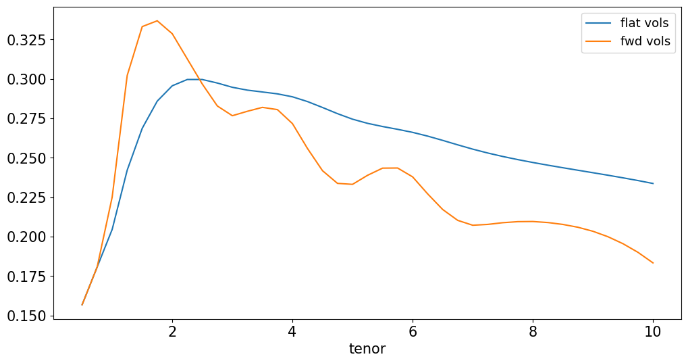
\includegraphics[width=0.9\linewidth,height=0.55\textheight,keepaspectratio]{figures/L6_1_c58_flat_vs_fwd.png}\end{center}

The blue line is the flat vol quoted by the market for caps of
tenors $0.5, 1, 2, \ldots, 10$~years. The orange line is the implied
forward vol of each new caplet, recovered by the bootstrap. Both
peak around tenor~$2$ at roughly $33\%$ and fall off thereafter; the
forward-vol line oscillates more aggressively because it is
maturity-resolved.
\end{keyblock}

The shape relationship is the same arithmetic that links YTMs to spot
rates: when the flat vol is rising in $T$, the new caplet must have a
forward vol \emph{higher} than the running flat vol to pull the
average up; when the flat vol is falling in $T$, the new caplet must
have a forward vol \emph{lower} than the running flat vol. The
lecturer made the class read this off the picture: ``as I see these
flat vols going up and up and up, what do I know must be true of
these caplet vols, of the forward vols? They have to be even higher.''

\begin{tipblock}
\textbf{Filling the gap.} The bootstrap is exactly identified. A
question from the class: should we worry about an over-identified
system, the way we did with the Treasury bootstrap in Week~1? No ---
caps and floors are OTC, the market quotes any tenor a buyer wants
(``you say, well, I only really like round numbers.\ I don't think
you're going to last long''), so for any quarterly grid there is
exactly one cap quote per tenor and exactly one new caplet whose
forward vol is unknown. The mechanical recursion always identifies
exactly one number from one equation.
\end{tipblock}

\subsection{Why we wanted the forward vols: pricing other
products}\label{L6-sec:why-fwdvol}

\begin{keyblock}
\textbf{What forward vols buy us.}
The forward vols are implied volatilities on \emph{forward interest
rates}: the $\sigma^{\text{fwd}}_{\tau}$ extracted from the cap at
tenor $\tau$ is the implied vol of the period-$1/n$ forward rate
locked at $\tau - 1/n$ and paid at $\tau$.
For pricing a different rate-derivative product (say, a callable
bond), what we typically need is the implied vol of \emph{some}
forward rate. The forward-vol curve from caps and floors gives us
a term structure of those implied vols on \emph{short-tenor}
(quarterly or semiannual) forward rates.
\end{keyblock}

The lecturer connected this directly back to the Freddie~Mac case
study: ``where did we see this before?\ We really needed an implied
vol on a forward rate.\ Where? Callable bonds.\ \ldots\ It would be
good enough to have an implied vol on the three-year forward interest
rate.''
The forward-vol curve from caps doesn't quite cover that, because the
caps give us implied vols on quarterly rates, not on a 2-year rate
locked three years out. ``It wasn't giving me info about the rate on
a two-year bond, whereas the swaption is going to do that.''
This is the cliffhanger that motivates the move to swaptions: caps
and floors give us forward vols on \emph{short} forward rates;
swaptions will give us forward vols on \emph{long} forward swap
rates, which is what you actually need to price options on long-dated
underlyings.

\section{Black vs Bachelier and the ATM convention}\label{L6-sec:blackbachelier}

\begin{keyblock}
\textbf{Cell \emph{``Normal'' quotes}.}
\emph{(Bachelier in addition to Black.)}\\
Black's formula assumes lognormal dynamics on the forward rate: the
rate cannot go negative. In recent years, with rates near zero and
with episodes of negative rates in some currencies (and of negative
prices in some commodities, e.g.\ March~2020 oil), normal-dynamics
models such as Bachelier's have become standard. Bloomberg quotes vols
in both flavours --- by default in the normal (Bachelier) form, with
a toggle for the lognormal (Black) form.\\
Conversion (ATM only):
\[
  \sigma_B \;=\; \sigma_N \,/\, f,
\]
where $f$ is the forward rate, $\sigma_B$ is the Black (lognormal)
vol, and $\sigma_N$ is the normal (Bachelier) vol. For OTM strikes
the conversion needs an adjustment; see the SABR-related literature
(Hagan, etc.).
\end{keyblock}

The lecturer emphasized that the choice between Black and Bachelier
is a modeling artistry question, not a doctrinal one. ``Whether
log-normal or normal is not totally obvious, which would be a better
model.'' If rates are very near zero the lognormal model wants a lot
of probability mass at low rates; if rates are around 4--5\% the
normal model gives a richer set of probabilities for the range you
are actually in (at the cost of a small probability mass on the
negative side). And neither is right: ``some artistry here, because
neither of these distributions is going to be quite right.''

The pragmatic take-away: Bloomberg's default is normal, the data the
class will be handed in the homework has been pre-converted to Black,
and the conversion formula is small enough not to affect dollar
prices materially.

\begin{keyblock}
\textbf{ATM, again.}
The at-the-money strike for a cap, floor, or swaption is \emph{not}
today's spot rate; it is the relevant \emph{forward} rate. For a
$T$-tenor cap, the ATM strike is the $T$-tenor swap rate (the rate
that makes the corresponding swap a zero-cost trade today). For a
swaption, the ATM strike is the forward swap rate; we will define
that precisely below.
\end{keyblock}

The lecturer reminded the class of the equity analog: in a Black
formula world without dividends, ATM means $K = F$, not $K = S$.
Move to fixed income and the same logic gives ATM = forward rate, not
spot rate. ``We should really be comparing the strike to the forward
price of the share in the case of dividends. So Black--Scholes
assumes no dividends \ldots\ and so in an intro options class, you
get used to the idea that at-the-money means strike equals today's
price. \ldots\ Here we need that same thing.'' The natural choice
of ATM strike for a $T$-tenor cap is the $T$-tenor (spot) swap
rate, because that is exactly the strike at which the long-cap,
short-floor portfolio replicates a zero-NPV swap.

\section{Swaps and swaptions}\label{L6-sec:swaptions}

\subsection{Swap refresher}\label{L6-sec:swap-refresh}

\begin{keyblock}
\textbf{Cell (Page \emph{Swaptions} \textperiodcentered{}
\emph{Swap}).}
\emph{(Already covered, but re-anchored here.)}\\
A receiving-fixed swap pays
\[
  \text{swap cashflow}_{T_i} \;=\; \frac{100}{n}\,\bigl(K - r_{T_{i-1}, T_i}\bigr),
\]
where $K$ is the (constant) swap rate, $r_{T_{i-1}, T_i}$ is the
floating rate set in arrears (locked at $T_{i-1}$, paid at $T_i$),
and the receiving-fixed party gets a positive cash flow when the
floating rate is below the swap rate. A swap is replicated as long a
fixed bond and short a floating-rate bond, and (Lecture~5) is
priced by no-arbitrage off the discount curve --- no derivative-pricing
machinery required.
\end{keyblock}

\subsection{Swaption definitions}\label{L6-sec:swaption-defs}

\begin{keyblock}
\textbf{Cells \emph{Swaptions}.}
\emph{(Two swaptions, two perspectives.)}
\begin{itemize}
  \item A \textbf{receiver swaption} is a contract today, with a
        premium paid today, that gives the holder the option (not
        obligation) at expiration $T_o$ to enter a swap
        \emph{receiving} the swap rate $K$ from $T_o$ to $T_o + T$.
        The receiver swaption is like a \emph{put} on a swap: it
        pays off when rates move \emph{down} (so the swap rate at
        $T_o$ is below $K$ and the holder collects the difference).
  \item A \textbf{payer swaption} is the option to enter the same
        swap \emph{paying} fixed; like a \emph{call} on a swap, it
        pays off when rates move \emph{up}.
  \item Being \emph{short} a receiver swaption is \emph{not} the same
        as being \emph{long} a payer swaption.
\end{itemize}
\end{keyblock}

The lecturer made the four-position grid explicit, the same way an
introductory options class would. ``You can be long the call, short
the call, long the put, short the put. They're all different. Same
thing here. You can be long the receiver swaption, short the receiver
swaption, long the payer swaption, short the payer swaption. They're
all different.''

\begin{keyblock}
\textbf{Three dates.}
A swaption involves three dates:
\begin{enumerate}[label=(\arabic*)]
  \item $T_o$ --- the swaption \emph{expiration}, when the option
        decision is made;
  \item $T_o$ --- the underlying swap's \emph{start} date (for plain
        swaptions, equal to $T_o$);
  \item $T_o + T$ --- the underlying swap's \emph{end} date.
\end{enumerate}
A ``$1Y \to 10Y$'' swaption has $T_o = 1$~year and underlying swap
tenor $T = 10$~years. \\
\textbf{Midcurve} swaptions allow the swap start date to be after
$T_o$ (e.g., $6m \to 1Y \to 5Y$); for our purposes, plain swaptions
with start = expiration are the default.
\end{keyblock}

The lecturer worked one numerical example by hand to anchor the
intuition. ``I'm going to enter into you a swaption where I want to
receive $4\%$ from you in this swap.\ A year from now, what if the
swap rate is $3\%$?'' The receiver gets to receive $4\%$ on a swap
the rest of the market is currently doing at $3\%$, so the receiver
exercises and locks in a positive spread on a 10-year stream. ``If
the rate's gone up to $5\%$ for 10-year swaps, I have an option to
enter with him to receive $4\%$. It's junk. I'm not going to exercise
it.'' Hence: receiver swaption is the put.

\subsection{Swaptions as the option toolkit on \emph{forward} swaps}\label{L6-sec:swaption-fwd}

A student wondered whether swaptions are ``redundant,'' since long-cap-short-floor already replicates a swap. The lecturer's answer
hinges on which kind of swap the parity replicates.

\begin{keyblock}
\textbf{Three put-call parities.}
\begin{center}
\begin{tabular}{l|l|l}
\textbf{Parity} & \textbf{LHS} & \textbf{RHS} \\
\hline
caplet $-$ floorlet & at strike $K$ & paying-fixed FRA at $K$ \\
cap $-$ floor & at strike $K$ & paying-fixed (spot) swap at $K$ \\
payer swaption $-$ receiver swaption & at strike $K$ & forward swap at $K$, settled at $T_o$ \\
\end{tabular}
\end{center}
At-the-money for each line means $K$ equals the relevant forward
rate: the FRA forward rate, the spot swap rate, the forward swap
rate.
\end{keyblock}

The crucial cell is the third line: \emph{payer minus receiver
swaption equals a forward swap}. The cap-floor pair already replicates
a \emph{spot} swap, but the payer-receiver swaption pair replicates a
\emph{forward} swap (a swap to be entered at $T_o$ at a rate locked
today). Forward swaps are themselves a real product --- ``a
significant market for a forward swap'' --- and swaptions are the
call/put primitives that decompose them.

\begin{checkpoint}
\textbf{My note.} The structural picture the lecturer wants recorded:
caps/floors decompose \emph{spot swaps} into asymmetric pieces;
swaptions decompose \emph{forward swaps} into asymmetric pieces.
Both products exist because the underlying (spot swap or forward
swap) is itself a major OTC market, and a market that big needs a
call/put toolkit on top of it. The way the lecturer drove the point
home: ``the same way you don't question, there might be interest in
having puts and calls on Tesla. Well, why? You could already go long
Tesla. You could short Tesla. \ldots\ You can build all sorts of
asymmetries.\ You can get leverage on what happens to Tesla through
this.''
\end{checkpoint}

\subsection{Caps vs swaptions: option-on-portfolio vs portfolio-of-options}\label{L6-sec:caps-vs-swaptions}

The lecturer ran a careful side-by-side that the class will return to
in the swaption-pricing exercise. Consider a $0.5Y \to 10Y$ semiannual
receiver swaption struck at the swap rate $K$, vs a $10.5Y$ floor
also struck at $K$, with the floor's first floorlet (at $T_1 = 0.5$)
included. Same dates, same payments, same strike --- but very
different products.

\begin{keyblock}
\textbf{Cell \emph{Forward Vols} (Page 7.2).} \emph{(The structural
distinction.)}
\begin{itemize}
  \item A \textbf{cap or floor} is a \emph{portfolio of options on
        single payments}. Each floorlet can be exercised independently
        every period; over the life of the floor the holder picks and
        chooses which periods to exercise.
  \item A \textbf{swaption} is a \emph{single option on a portfolio
        of payments}. One exercise decision at $T_o$; from then on
        the holder is committed for the full swap term.
\end{itemize}
The floor is therefore worth (weakly) \emph{more} than the swaption
with the same payments. Optionality on each individual cash flow
beats optionality on the bundle.
\end{keyblock}

The lecturer's framing: ``the way they work in practice is what
they're good at hedging and decomposing.\ The swaptions are perfect
for inferring and decomposing the forward swap.\ The caps and floors
are perfect for decomposing and inferring the spot swaps.''
This perspective will determine which product the trader uses to
extract a given forward vol: caps and floors for spot-swap-flavored
forward vols (short tenor, periodic payments), swaptions for
forward-swap-flavored forward vols (long tenor, single exercise
decision).

\begin{checkpoint}
\textbf{My note.} A more practical implication that the lecturer
flagged near the end: at any given moment, the cap-floor model and
the swaption model that traders actually use are mathematically
\emph{inconsistent} with each other. Both are commercial models on
top of Black-flavored or Bachelier-flavored quoting; they happen to
disagree on cross-market vols at a level small enough that traders
``get along,'' but every market participant has to make a choice on
Bloomberg's volcube screen --- pull vols from caps/floors or from
swaptions --- and the choice has consequences downstream. The exact
analog of the swap curve vs the Treasury curve dispute (Lecture~4):
two consistent worlds that just don't quite agree.
\end{checkpoint}

\section{Black's formula for swaptions}\label{L6-sec:swaption-black}

\begin{keyblock}
\textbf{Cells \emph{Black's Formula for Swaptions}.}
\emph{(One Black call, scaled by the swap discount factor.)}\\
Use Black's formula for a European swaption with the following
adjustments:
\begin{itemize}
  \item \textbf{Underlying:} the \emph{forward swap rate}
        $f_n(0, T_o, T)$ replaces the underlying rate (defined
        below).
  \item \textbf{Time:} use $\tau = T_o$ as the variance accrual time
        \emph{and} the discount time. Unlike the caplet, where
        uncertainty resolves $1/n$ before payment, the swaption
        resolves all of its uncertainty at the swaption expiration
        $T_o$.
  \item \textbf{Discount factor:} replace $Z(0, T_o)$ by the
        \emph{swap discount factor}
        \[
          Z^{\text{swap}}(0, T_o, T) \;\equiv\; \sum_{i = 1}^{m} Z(0, T_i),
        \]
        where $T_i$ are the swap payment dates of the underlying
        swap, $T_m = T_o + T$. This sum scales the formula to
        reflect that exercising the swaption commits the holder to
        $m$ payments instead of one.
\end{itemize}
The payer swaption (option to pay fixed) is a Black call;
the receiver swaption (option to receive fixed) is a Black put. With
the substitutions above:
\[
  p_{\text{payer}} \;=\; \frac{100}{n}\,Z^{\text{swap}}(0, T_o, T)\,
        \Bigl[\, f_n\,\cN(d_1) \;-\; K\,\cN(d_2)\,\Bigr],
\]
\[
  p_{\text{receiver}} \;=\; \frac{100}{n}\,Z^{\text{swap}}(0, T_o, T)\,
        \Bigl[\, K\,\cN(-d_2) \;-\; f_n\,\cN(-d_1)\,\Bigr],
\]
\[
  d_1 \;=\; \frac{\ln(f_n / K) + \tfrac{1}{2}\,\sigma^2\,T_o}{\sigma\,\sqrt{T_o}},
  \qquad
  d_2 \;=\; d_1 - \sigma\,\sqrt{T_o}.
\]
\end{keyblock}

The lecturer pointed out the conceptual gain. With caps, every
caplet had its own expiration, its own forward, and (in principle)
its own forward vol; pricing a cap meant looping. With a swaption,
every payment of the underlying swap responds to the same option
exercise decision, so each payment shares the same forward swap rate
and the same time-to-expiration. ``A swaption is a single option,
but it involves (if exercised) multiple payments.\ Unlike the cap,
each payoff of the exercised swaption corresponds to the same
option, and thus is priced identically in Black's formula. The only
adjustment is to discount the exercised payoffs appropriately,
reflecting that they have different maturities.''

\begin{tipblock}
\textbf{Filling the gap.} Why does the swap-discount-factor sum work
as a numeraire substitute? The clean justification (which the
lecturer flagged but did not derive in class) is a measure change:
under the so-called \emph{annuity measure} associated with the
numeraire $Z^{\text{swap}}(0, T_o, T)$, the forward swap rate is a
martingale, and the standard Black derivation goes through with
$Z^{\text{swap}}$ in place of $Z$. The replication argument is the
content of the change-of-numeraire result from FINMAT~330. ``Trust
me, this will turn out to be a valid numeraire that will give us
martingale pricing and you can just go ahead and use it.''
\end{tipblock}

\subsection{The forward swap rate}\label{L6-sec:fwd-swap-rate}

\begin{keyblock}
\textbf{Cell \emph{Discount Factor Formula} (Page 7.2).}
\emph{(The forward swap rate.)}
\[
  f_n(t, T_{\text{fwd}}, T) \;\equiv\; n\,
        \frac{Z(t, T_{\text{fwd}}) \;-\; Z(t, T)}{\sum_{i = 1}^{m} Z(t, T_i)},
\]
where $T_i$ ($1 \le i \le m$) are the underlying swap's payment
dates with $T_m = T$, $T_{\text{fwd}}$ is the swap start date, and
$n$ is the swap's payment frequency ($n = 2$ for semiannual,
$n = 4$ for quarterly, etc.).
The forward swap rate is the strike at which the forward swap
(commit-now-to-swap-later) has zero NPV.
\end{keyblock}

The formula is the one the class derived (in a different notation) in
Lecture~4 for spot swap rates: the swap rate is the constant fixed
rate that, when applied to a notional of $100$ at frequency $n$ over
the swap's payment dates, present-values to the same total as the
floating leg. The numerator
$Z(t, T_{\text{fwd}}) - Z(t, T)$ is the present value of the floating
leg of a forward swap (initial face $100$, return of face at maturity,
floating coupons in between with present value $100 \cdot [Z_{\text{fwd}}
- Z_T]$ in the appropriate units); the denominator
$\sum_i Z(t, T_i)$ is the present value annuity of one dollar at the
swap's payment dates.
The lecturer made the point that ``calculating forward rates from
spot rates is done as usual, the same as for treasury rates'' --- if
you have today's swap discount curve, you have everything you need to
compute the forward swap rate without any vol input.

\begin{tipblock}
\textbf{Filling the gap.} For a $1Y \to 2Y$ annual swaption (so
$T_o = 1$, $T = 3$, payments at $T_i = 2, 3$), the forward swap rate
is
\[
  f_2(0, 1, 3) \;=\; 1 \cdot \frac{Z(0, 1) - Z(0, 3)}{Z(0, 2) + Z(0, 3)}.
\]
And the swap discount factor is $Z^{\text{swap}}(0, 1, 3)
= Z(0, 2) + Z(0, 3)$. The lecturer worked through this exact example
on the slide.
\end{tipblock}

\subsection{Why we want swaption-implied vols}\label{L6-sec:why-swaption-vol}

The lecturer brought the chapter back to the original motivation. We
want vols, not just prices, because vols are the apples-to-apples
quoting language across rate-derivative products. ``We can get a
forward swap rate without any word of swaptions.\ \ldots\ But none of
that would have given us vols on these things.\ Now, why do we want
those vols so much? Because our game here is not to just use
swaptions to price swaptions, that would be pointless.''

The downstream applications: callable bonds (need an implied vol on a
forward bond rate), mortgage-backed securities (need an implied vol
on a long-tenor forward rate), exotic interest-rate options. Caps and
floors don't reach the long-tenor forward rates that callables and
MBS need; swaptions do. ``A swaption is going to be a very nice way
to infer what is the implied vol on something used for, say, the
Freddie~Mac callable.\ \ldots\ Whereas the cap and floor wouldn't be
our best option there, because that is going to give us a forward
rate over what term? Over a quarter.''

The Bloomberg \emph{volcube} screen (the lecturer's term) is the
default tool for pulling these vols, and it has a top-level toggle:
caps/floors or swaptions. The choice is the same kind of branch point
the class faced when picking a discount curve in Lecture~4.

\section{Closing remarks and assigned exercises}\label{L6-sec:close}

The lecturer announced three exercises for the week and previewed a
case study.

\begin{exerciseblock}
\textbf{Exercise (assigned). Cap stripping.} Given a Bloomberg cap
quote sheet (flat vols at quarterly tenors out to $T = 10$), strip
out the implied caplet prices and forward vols. Use the bootstrap
described in \S\ref{L6-sec:stripping}, and produce the flat-vs-forward
plot of the type shown in cell~58 of \emph{7.1}. Confirm that the
flat-vol curve is monotonically increasing then decreasing in tenor,
and that the forward-vol curve oscillates more aggressively but
matches in level at $T = 0.5$.
\end{exerciseblock}

\begin{exerciseblock}
\textbf{Exercise (assigned). Swaption pricing.} Given Bloomberg
swaption data from June 2025 (expiry $T_o$, swap tenor $T$, ATM
implied vols $\sigma$):
\begin{enumerate}[label=(\arabic*)]
  \item Compute the forward swap rate $f_n(0, T_o, T)$ from the
        provided swap rates, discount factors, and forward rates.
  \item Compute the swap discount factor
        $Z^{\text{swap}}(0, T_o, T) = \sum_i Z(0, T_i)$ over the
        underlying swap's payment dates.
  \item Price the payer swaption and the receiver swaption via Black's
        formula with $K = $ the ATM forward swap rate.
  \item Repeat across $(T_o, T)$ pairs --- the lecturer wants the
        class to focus on the $1Y \to 4Y$ swaption (i.e.\ $T_o = 1$,
        $T = 4$, quarterly payments) but also the $3m \to 4Y$,
        $2Y \to 4Y$, and $1Y \to 2Y$ alternates. Do all calculations
        at the ATM strike only.
\end{enumerate}
The exercise also previews skew (different strikes at the same
$(T_o, T)$); the lecturer's caveat is that swaption liquidity
collapses sharply outside ATM, so the ATM cross-section is the
business-relevant focus.
\end{exerciseblock}

\begin{exerciseblock}
\textbf{Case study (forthcoming). Capped floaters.} The lecturer
flagged but did not yet hand out a case study on capped floaters ---
floating-rate notes whose floating coupon is capped at a maximum
rate. The case is loosely related to the 1994 Orange County
bankruptcy on \emph{leveraged inverse floaters}, though the precise
product differs. The lecturer's tease: ``these products have real-
world use and can go really bad if you don't understand them.'' The
case will be handed out by Canvas announcement once the dataset is
finalized; pending that, the cap-stripping and swaption-pricing
exercises are the homework for the week.
\end{exerciseblock}

\subsection{Recap of what changed in our toolkit}\label{L6-sec:recap}

The lecture adds three new objects to the rate-derivatives toolkit:

\begin{enumerate}[label=(\arabic*)]
  \item \textbf{Forward volatility.} The implied vol of a forward
        rate, recovered from cap quotes by bootstrap. Forward vols are
        the consistent maturity-by-maturity vols; flat vols are the
        bundled YTM-style quote sitting on top.
  \item \textbf{Black's formula for swaptions.} One Black call (or
        put) on the forward swap rate, scaled by the swap discount
        factor $\sum_i Z(0, T_i)$ rather than a single payment-date
        $Z(0, T)$. The variance accrual time is $T_o$, not
        $T_o - 1/n$ --- there is no time-mismatch on a swaption.
  \item \textbf{The forward swap rate.} A direct generalization of
        the forward rate to swaps; computed from the discount curve
        alone, without any vol input.
\end{enumerate}

The structural picture the lecturer wants the class to leave with:
caps, floors, and swaptions are the call/put toolkit for the swap
world. Caps and floors strip a spot swap into asymmetric pieces;
swaptions strip a forward swap into asymmetric pieces. Implied
volatility on these products is a quoting language, the same way YTM
is a quoting language on bonds; the consistent objects underneath
(forward vols, forward swap rates) are what actually feed downstream
applications --- callable bonds, mortgage-backed securities, exotic
rate options. Lecture~7 turns to the cross-section of strikes
(volatility skew), where the quoting-language abstraction starts to
fray and SABR-style models replace plain Black.
